\documentclass{report}
\usepackage[T1]{fontenc}
\usepackage{graphicx}
\usepackage{graphics}

\usepackage{xcolor}
\newcommand\comment[1]{\textcolor{red}{#1}}
% tikz
\usepackage{tikz-cd}
\usepackage{tikz}
\usetikzlibrary{fit,positioning,shapes.geometric, arrows}
\usepackage{subcaption}

\usepackage{enumitem}
\usepackage{pdflscape}


\usepackage{amsmath}
\usepackage{adjustbox}
\usepackage{stmaryrd}
\usepackage{listings}

\usepackage{pdflscape}
\usepackage{array}
\usepackage{longtable}



\usepackage{multicol}
\usepackage{holindex}
\usepackage{proof}

\setHOLlinewidth{50}
\useHOLfile{report.hdf}

\title{Technical Report\\Formalizing GP\,2 in HOL4}
\author{Robert S\"oldner  \qquad Detlef Plump}

\begin{document}

\maketitle
\tableofcontents

\chapter{Lexing and Parsing}

\chapter{Graphs and Morphisms}
We model finite graphs and allow parallel edges and loops.

\section{Hostgraph}
\blockHOLthm{hostgraph.datatype_nodemark}
\blockHOLthm{hostgraph.datatype_edgemark}
\blockHOLthm{hostgraph.datatype_label}
\blockHOLthm{hostgraph.datatype_hostgraph}

The well-formed predicate is given by
\blockHOLthm{hostgraph.wf_hostgraph_def}
Here, the item_uniqueness propert \citeHOLthm{hostgraph.item_uniqueness_def} expresses, that
node and edge its are unique.

\section{Rulegraph}
\blockHOLthm{rulegraph.datatype_nodemark}
\blockHOLthm{rulegraph.datatype_edgemark}
\blockHOLthm{rulegraph.datatype_label}
\blockHOLthm{rulegraph.datatype_rulegraph}

The well-formed predicate is given by
\blockHOLthm{rulegraph.wf_rulegraph_def}

\chapter{Semantics}

\section{Label Semantics}
\blockHOLthm{eval_label_ConstInt_rule}
\blockHOLthm{eval_label_ConstString_rule}
\blockHOLthm{eval_label_ConstChar_rule}
\blockHOLthm{eval_label_Nil_rule}
\blockHOLthm{eval_label_VarBound_rule}
\blockHOLthm{eval_label_Outdeg_rule}
\blockHOLthm{eval_label_Indeg_rule}
\blockHOLthm{eval_label_LengthInt_rule}
\blockHOLthm{eval_label_LengthString_rule}
\blockHOLthm{eval_label_LengthChar_rule}
\blockHOLthm{eval_label_Add_rule}
\blockHOLthm{eval_label_Sub_rule}
\blockHOLthm{eval_label_Mult_rule}
\blockHOLthm{eval_label_Div_rule}
\blockHOLthm{eval_label_Negate_rule}
\blockHOLthm{eval_label_Concat_rule}
\blockHOLthm{eval_label_Empty_rule}
\blockHOLthm{eval_label_Cons_rule}

\section{Condition Semantics}
\blockHOLthm{eval_condition_edgeTest}
\blockHOLthm{eval_condition_edgeTestLabel}
\blockHOLthm{eval_condition_subType}
\blockHOLthm{eval_condition_condLabelEq}
\blockHOLthm{eval_condition_condLabelNeq}
\blockHOLthm{eval_condition_condLabelGt}
\blockHOLthm{eval_condition_condLabelGteq}
\blockHOLthm{eval_condition_condLabelLt}
\blockHOLthm{eval_condition_condLabelLteq}
\blockHOLthm{eval_condition_condAnd}
\blockHOLthm{eval_condition_condOr}
\blockHOLthm{eval_condition_condNot}

\section{Rule instantiation}

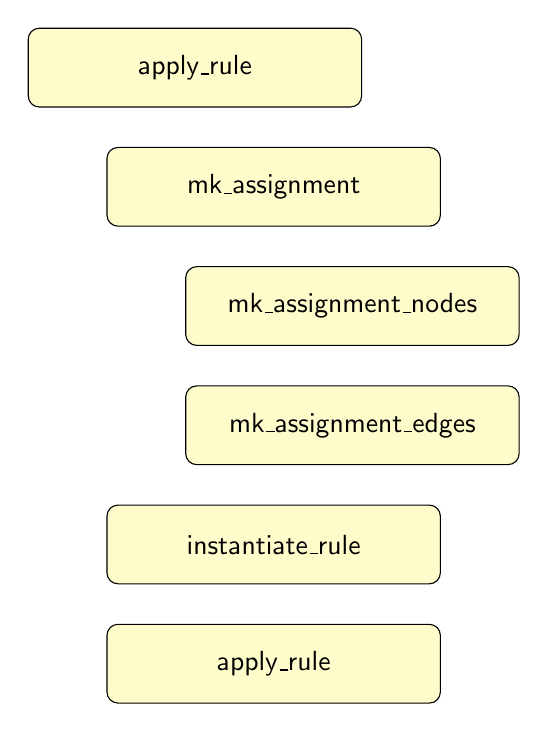
\begin{tikzpicture}[
  node distance=0.5cm and 1cm,
  stage/.style={rectangle, draw, fill=yellow!20, rounded corners, text width=4cm, align=center, minimum height=1cm},
  note/.style={rectangle, draw=gray, fill=gray!10, text width=5cm, align=left, font=\small},
  arrow/.style={-{Stealth}, thick},
  every node/.style={font=\sffamily}
]
\node[stage] (start) {apply\_rule};
\node[stage, below=of start, xshift = 1cm] (assign) {mk\_assignment};

\node[stage, below=of assign, xshift = 1cm] (assign_nodes) {mk\_assignment\_nodes};
\node[stage, below=of assign_nodes] (assign_edges) {mk\_assignment\_edges};

\node[stage, below=of assign_edges, xshift = -1cm] (instantiate) {instantiate\_rule};
\node[stage, below=of instantiate] (instantiate) {apply\_rule};

% \node[stage, below=of assign] (nodes) {mk\_assignment\_nodes};
% \node[stage, below=of nodes] (unify) {unify\_nodeattr};
% \node[stage, below=of unify] (edges) {mk\_assignment\_edges};
% \node[stage, below=of edges] (instantiate) {instantiate\_rule};
% \node[stage, below=of instantiate] (lhsrhs) {instantiate\_rulegraph (lhs/rhs)};
% \node[stage, below=of lhsrhs] (eval) {eval\_label\_fun / eval\_mark};
% \node[stage, below=of eval] (apply) {apply\_ruleinstance};

% % Arrows
% \draw[arrow] (start) -- (assign);
% \draw[arrow] (assign) -- (nodes);
% \draw[arrow] (nodes) -- (unify);
% \draw[arrow] (unify) -- (edges);
% \draw[arrow] (edges) -- (instantiate);
% \draw[arrow] (instantiate) -- (lhsrhs);
% \draw[arrow] (lhsrhs) -- (eval);
% \draw[arrow] (eval) -- (apply);

% % Notes
% \node[note, right=3cm of start] {Top-level entry point. Takes rule, morphism, and host graph.};
% \node[note, right=3cm of assign] {Initial assignment computation by matching LHS nodes/edges.};
% \node[note, right=3cm of nodes] {Iterates over LHS node IDs and attempts to match each with host node.};
% \node[note, right=3cm of unify] {Checks mark compatibility; label unification not yet implemented.};
% \node[note, right=3cm of edges] {Matches LHS edge attributes with hostgraph edges.};
% \node[note, right=3cm of instantiate] {Checks condition and evaluates lhs/rhs under the assignment.};
% \node[note, right=3cm of lhsrhs] {Maps and evaluates rulegraph nodes/edges via assignment.};
% \node[note, right=3cm of eval] {Evaluates label expressions and computes derived values.};
% \node[note, right=3cm of apply] {Applies rule instance to host graph. Performs the actual rewriting.};

\end{tikzpicture}



\section{Context Conditions}

\begin{landscape}
\begin{longtable}{m{4cm} | m{11cm} | m{4cm}}
Name & Description & Note \\
\hline
Identifier Length & Identifiers have a maximum length of 63 characters. & Enforced by lexer.\\
Reserved Words & GP\,2 keywords must not be used as identifiers. & Enforced by lexer.\\
Main Declaration & There is exactly one main declaration in a single program. & \citeHOLthm{program.has_main_entry_def}\\
Unique Procedure Names & Each procedure name must not be used in more than one procedure declaration. & Enforce by ML.\\
Rule Declaration Scope & Each rule name must not be used in more than one declaration in the same scope. & Enforce by ML.\\
Rule Call Validity & Any name in a rule call must belong to a rule declared in a visible scope. & \citeHOLthm{program.rule_call_validity_def}\\
Procedure Call Validity & Any name in a procedure call must belong to a procedure declared in a visible scope. & \citeHOLthm{program.proc_call_validity_def}\\
Break & The break statement must only appread within a loop. If the break is in the condition of a branching statement, its containing loop must occur within the same condition. & \citeHOLthm{program.condition_break_def}\\
Variable Declarations 1 & Each type must appear at most once in a rules variable list. & Enforced by ML Code\\
Variable Declarations 2 & Variable IDs must be distinct in the declaration list of a rule. & Enforced by representation in HOL4. \\
Interface Nodes & Each node ID in the interface list must appear exactly once and must occur in both the left-hand side and the right-hand side. & \citeHOLthm{rule.wf_interface_def}\\
Bidirectional Edge 1 & A right-hand side bidirectional edge must be incident to the same two nodes as a left-hand side bidirectional edge. & \citeHOLthm{rule.bidir_edge_endpoint_agreement_def}\\
Bidirectional Edge 2 & There is at most one bidiretional edge between a pair of nodes. & \citeHOLthm{rulegraph.bidir_edge_uniqueness_def}\\
Node/Edge ID Uniqueness & Node IDs and edge IDs must be pairwise distinct within a single graph. \comment{Duplicate node and edge ids are not possible as we represent them as a set. Maybe check while parsing?} & \citeHOLthm{hostgraph.item_uniqueness_def} and \citeHOLthm{rulegraph.item_uniqueness_def}\\
Sources and Targets & The two node IDs in an edge declaration must match a node ID declared in the same graph. & \citeHOLthm{hostgraph.wf_hostgraph_def} and \citeHOLthm{rulegraph.wf_rulegraph_def}\\
Variable Consistency 1 & Any variable in a rule must be declared in the variable list of the associated rule. & \citeHOLthm{rule.variable_consistency1_def}\\
Variable Consistency 2 & Any variable in the right-hand side must be present in the left-hand side of the same rule. & \citeHOLthm{rule.variable_consistency2_def}\\
Grey and Dashed & Nodes must not be marked dashed and edges must not be marked grey & Enforced by lexer.\\
Wildcard Consistency & A right-hand side item with the mark any must be in the interface of the rule and its counterpart in the left-hand side must be a wildcard. & \citeHOLthm{rule.wildcard_consistency_def}\\
Well-typed expressions & Any expression in a label or condition must conform to the type grammar. & \citeHOLthm{rule.welltyped_rule_def}\\
Degree Operators & The argument of a degree operator (indeg or outdeg) must be a node ID occuring in the interface of its containing rule. & \citeHOLthm{rule.degree_op_consistency_def}\\
Simple Labels & Each expression in the left-hand side of a rule declaration must be a simple list. \comment{See HOL thm and Brians thesis. There are 3 items to check} & \citeHOLthm{rule.is_simple_rule_def} \\
Edge Predicate & Each node ID in an edge predicate must occur in the interface of its containing rule. & \citeHOLthm{rule.edge_pred_consistency_def}\\
Integer Comparisions & In a condition, the relation operators >, >=, <, <= must only be applied to integer expressions. & \citeHOLthm{rule.cond_typeof_rules} \\

\end{longtable}
\end{landscape}

% \chapter{Graph}
% Node and edge identifiers are represented using strings.
% Graphs are defined using predicate sets and finite maps as follows:
% \blockHOLthm{graph.datatype_graph}

% A wellformed graph has to satisfy the following predicate:
% \blockHOLthm{graph.wf_graph_def}

% We have two kinds of graphs: \emph{Hostgraphs} and \emph{Rulegraphs} which we define in the subsequent sections.
% \section{Hostgraph}
% Hostgraphs are used as the input graphs and we define the corresponding node and edge marks as follows:
% \blockHOLthm{graph.datatype_hostgraph_edge_mark}
% \blockHOLthm{graph.datatype_hostgraph_node_mark}
% The atoms are defined as follows:
% \blockHOLthm{graph.datatype_hostgraph_atom}
% TODO: change the list representation and bring it into the datatype

% We can further define the type for hostlabels:
% % \blockHOLty{hostlabel}

% \section{Rulegraphs}
% Here, we have an additional mark any:
% \blockHOLthm{graph.datatype_rulegraph_edge_mark}
% \blockHOLthm{graph.datatype_rulegraph_node_mark}

% Rulegraphs contain variables, which we represent using a string.

% \blockHOLthm{graph.datatype_rulegraph_atom}

% \chapter{Morphism}
% Morphisms are defined using a record type and two finite maps, mapping from node (edge) identifier to node (edge) identifier.
% \blockHOLthm{morphism.datatype_morphism}

% We define the source and target preservation property as follows:
% \blockHOLthm{morphism.preserve_source_def}
% \blockHOLthm{morphism.preserve_target_def}

% Furthermore, the defined rootedness property is expressed as:
% \blockHOLthm{morphism.preserve_defined_rootedness_def}


% \chapter{Rule}

% Rule parameters are types using the following types:
% \blockHOLthm{rule.datatype_ty}

% Application conditions are given by:
% \blockHOLthm{rule.datatype_cond}

% and the rule record is given by:
% \blockHOLthm{rule.datatype_rule}



% \chapter{Program}

% \chapter{Semantics}

% \chapter{Attributed DPO}

% \chapter{Pretty Printing}

% \chapter{Verification Examples}

\printLongHOLIndex


\bibliographystyle{splncs04}
\bibliography{report}

\end{document}
